\section{Chapter 11}
\subsection{11.1}
\begin{itemize}
    \item[2.] Which of these graphs are trees? \vspace{1mm}\\
          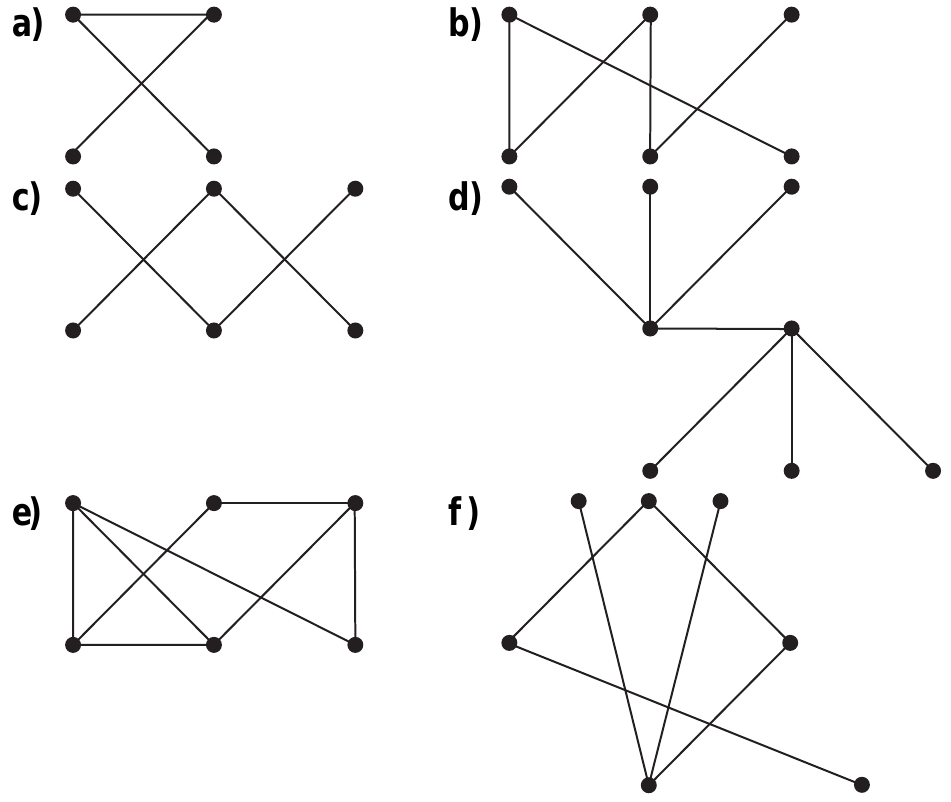
\includegraphics[scale = 0.4]{img/11_1_2_graphs.png} \\
          \answer
          \begin{tasks}(2)
              \task Tree
              \task Tree
              \task Not a tree
              \task Tree
              \task Not a tree
              \task Tree
          \end{tasks}
          \newpage
    \item[4.] Answer these questions about the rooted tree illustrated. \\
          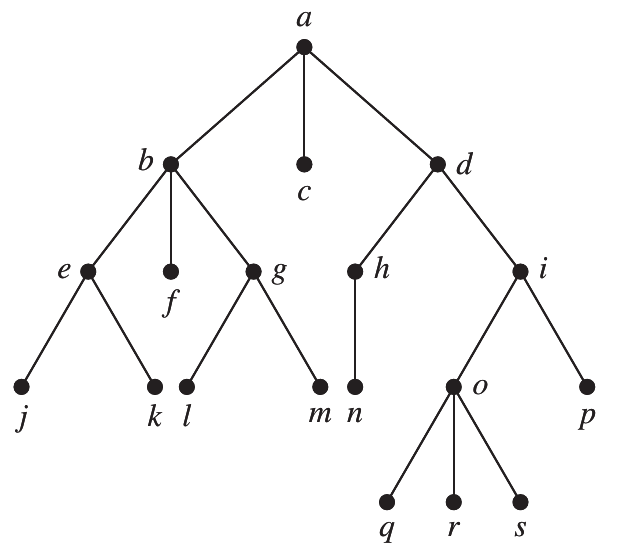
\includegraphics[scale = 0.5]{img/11_1_4_graph.png} \\
          \begin{enumerate}[a.]
              \item Which vertex is the root?
              \item Which vertices are internal?
              \item Which vertices are leaves?
              \item Which vertices are children of j ?
              \item Which vertex is the parent of h?
              \item Which vertices are siblings of o?
              \item Which vertices are ancestors of m?
              \item Which vertices are descendants of b?
          \end{enumerate}
          \answer
          \begin{enumerate}[a.]
              \item $a$
              \item $a, b, d, e, g, h, i, o$
              \item $c, f, j, k, l, m, n, p, q, r, s$
              \item $j$ has no children.
              \item $d$
              \item $p$
              \item $g, b, a$
              \item $e, f, g, j, k, l, m$
          \end{enumerate}

    \item[6.]  Is the rooted tree in Exercise 4 a full m-ary tree for some
          positive integer m? \\
          \answer \\
          No, it's not a full m-ary tree because there are some internal nodes who
          have a different ammount of children. For example, $b$ has 3 children but "i"
          only has 2.

    \item[10.]  Draw the subtree of the tree in Exercise 4 that is rooted
          at
          \begin{tasks}(3)
              \task a.
              \task c.
              \task e.
          \end{tasks}
          \answer
          \begin{tasks}(3)
              \task \text{}\\
              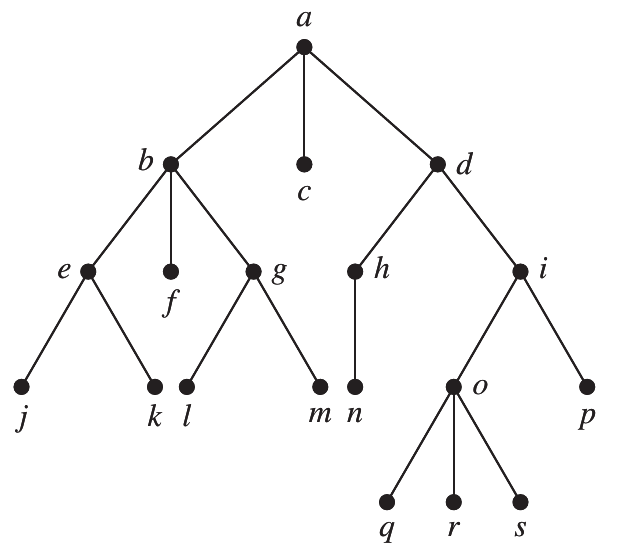
\includegraphics[scale = 0.35]{img/11_1_4_graph.png}

              \task \text{}\\
              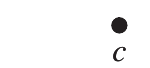
\includegraphics[scale = 0.5]{img/11_1_10b_graph.png}

              \task \text{}\\
              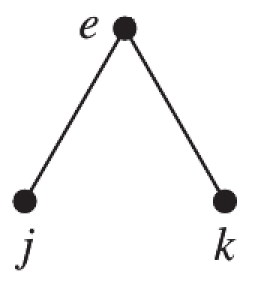
\includegraphics[scale = 0.4]{img/11_1_10c_graph.png}
          \end{tasks}

    \item[18.] How many vertices does a full 5-ary tree with 100 internal
          vertices have? \\
          \answer \\
          $n = mi + 1 = 5 \cdot 100 + 1 = 501$ vertices.

    \item[20.]  How many leaves does a full 3-ary tree with 100 vertices
          have? \\
          \answer \\
          $l = n - (n-1)/m = 100 - 99/3 = 67$ leaves.
\end{itemize}

\subsection{11.3}
\begin{itemize}
    \item[8.] Determine the order in which a preorder
          traversal visits the vertices of the given ordered rooted tree. \\
          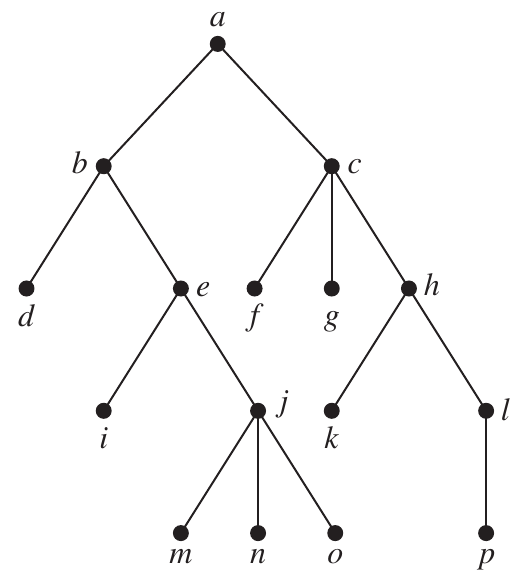
\includegraphics[scale=0.6]{img/11_3_8_tree.png} \\
          \answer \\
          \textit{a, b, d, e, i, j, m, n, o, c, f, g, h, k, l, p}

 \newpage

    \item[12.]  In which order are the vertices of this ordered rooted tree
          visited using an inorder traversal? \\
          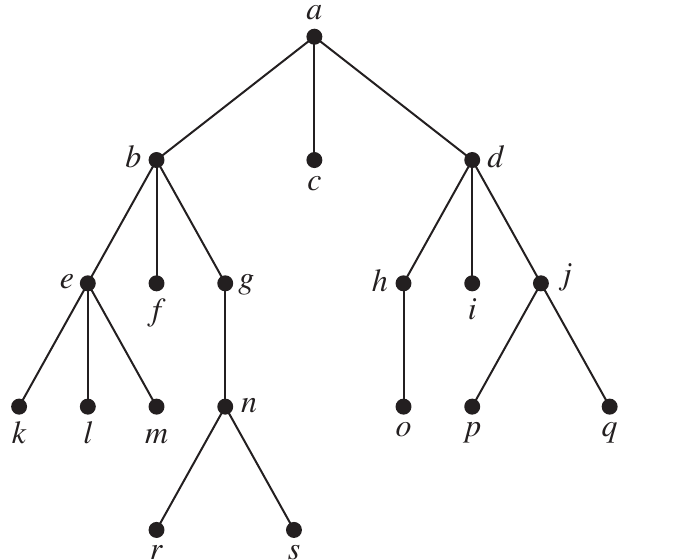
\includegraphics[scale=0.6]{img/11_3_12_tree.png} \\
          \answer \\
         \textit{k, e, l, m, b, f, r, n, s, g, a, c, o, h, d, i, p, j, q}

    \item[14.] In which order are the vertices of the ordered rooted tree
in Exercise 8 visited using a postorder traversal?\\
\answer \\
\textit{d, i, m, n, o, j, e, b, f, g, k, p, l, h, c, a}

\item[16.] 
\begin{enumerate}[a.]
\item Represent the expression $((x + 2) \uparrow 3) \cdot (y -(3 + x)) - 5$ using a binary tree.
\item Write this expression in prefix notation.
\item Write this expression in postfix notation.
\item Write this expression in infix notation.
\end{enumerate}
\answer \\
\begin{enumerate}[a.]
    \item \text{}\\
    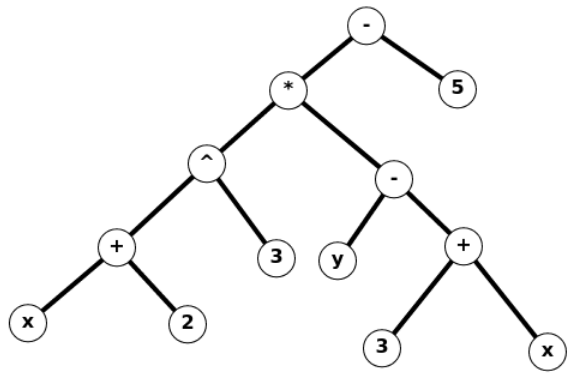
\includegraphics[scale = 0.7]{img/11_3_16_tree.png}
    \item - * $\uparrow$ + $x$ 2 3 - $y$ + 3 $x$ 5
    \item $x$ 2 + 3 $\uparrow$ $y$ 3 $x$ + - * 5 -
    \item $(((x + 2) \uparrow 3) \cdot (y -(3 + x))) - 5$
\end{enumerate}

\item[22.]  Draw the ordered rooted tree corresponding to each of
these arithmetic expressions written in prefix notation.
Then write each expression using infix notation.
\begin{enumerate}[a.]
\item + * + - 5 3 2 1 4
\item $\uparrow$ + 2 3 - 5 1
\item * / 9 3 + * 2 4 - 7 6
\end{enumerate}
\answer
\begin{enumerate}[a.]
    \item $(((5-3) + 2) \cdot 1) + 4 $ \\
    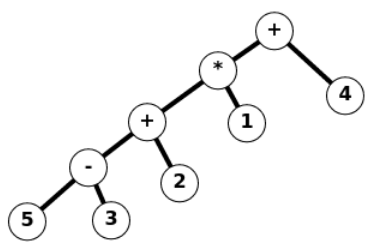
\includegraphics[]{img/11_3_22a_tree.png}
    \item $(2+3) \uparrow (5-1) $ \\
    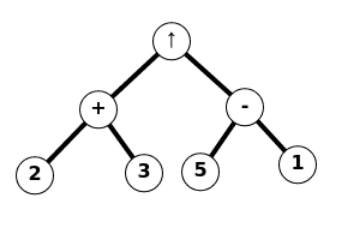
\includegraphics[]{img/11_3_22b_tree.png}
    \item $(9/3)*((2*4)+(7-6))$ \\
    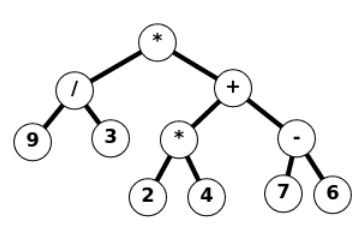
\includegraphics[]{img/11_3_22c_tree.png}
\end{enumerate}

\item[24.]  What is the value of each of these postfix expressions?
\begin{enumerate}[a.]
\item 5 2 1 - - 3 1 4 + + *
\item 9 3 / 5 + 7 2 - *
\item 3 2 * 2 $\uparrow$ 5 3 - 8 4 / * -
\end{enumerate}
\answer
\begin{enumerate}[a.]
    \item 32
    \item 40
    \item 32
\end{enumerate}
\end{itemize}

\subsection{11.4}
\begin{itemize}
    \item[4.] Find a spanning tree for the graph shown by 
    removing edges in simple circuits. \\
    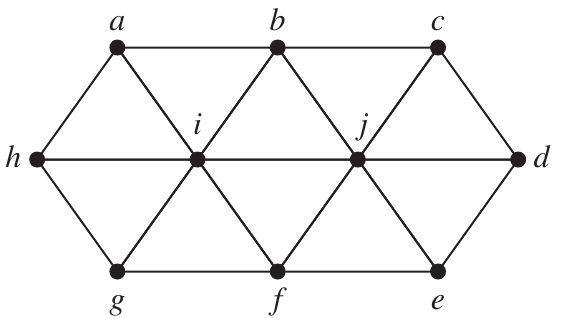
\includegraphics[scale=0.7]{img/11_4_4_graph.png} \\
    \answer \\
    \text{} \\
    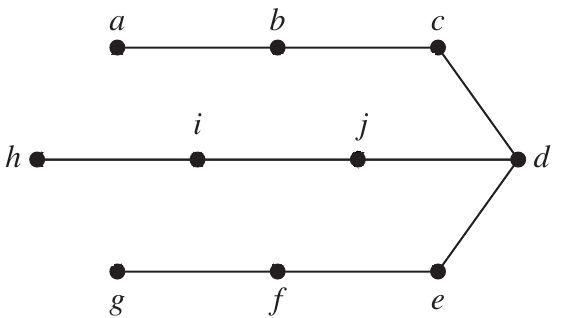
\includegraphics[scale=0.7]{img/11_4_4_tree.png}
\end{itemize}
For 8 and 10 draw all the spanning trees of the given
simple graph.
\begin{itemize}
\item[8.]  \text{}\\
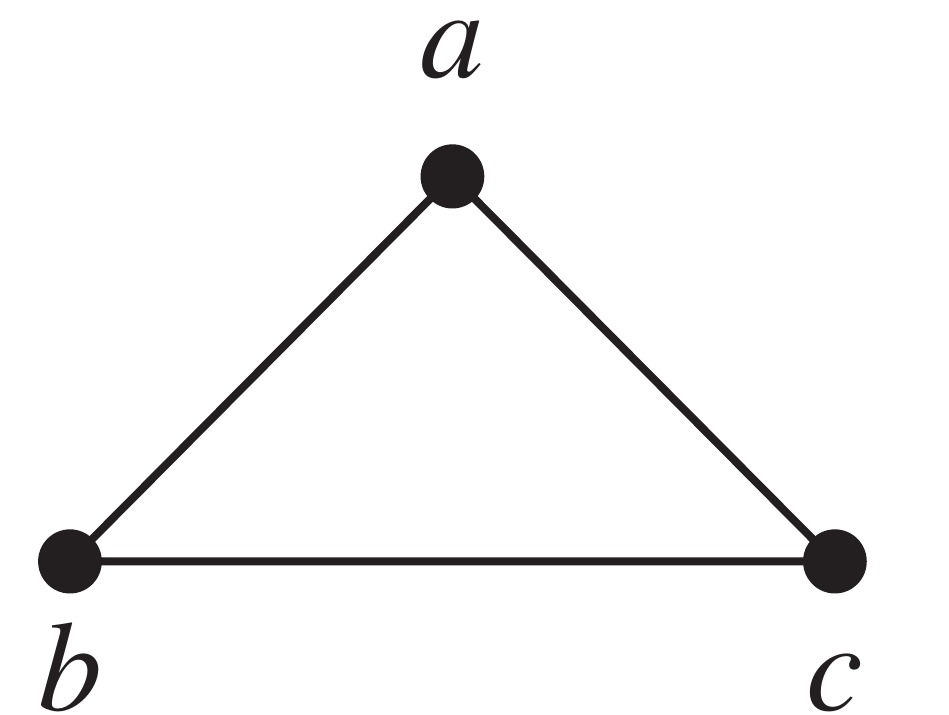
\includegraphics[scale = 0.2]{img/11_4_8_graph.png} \vspace{2mm} \\
\answer \\
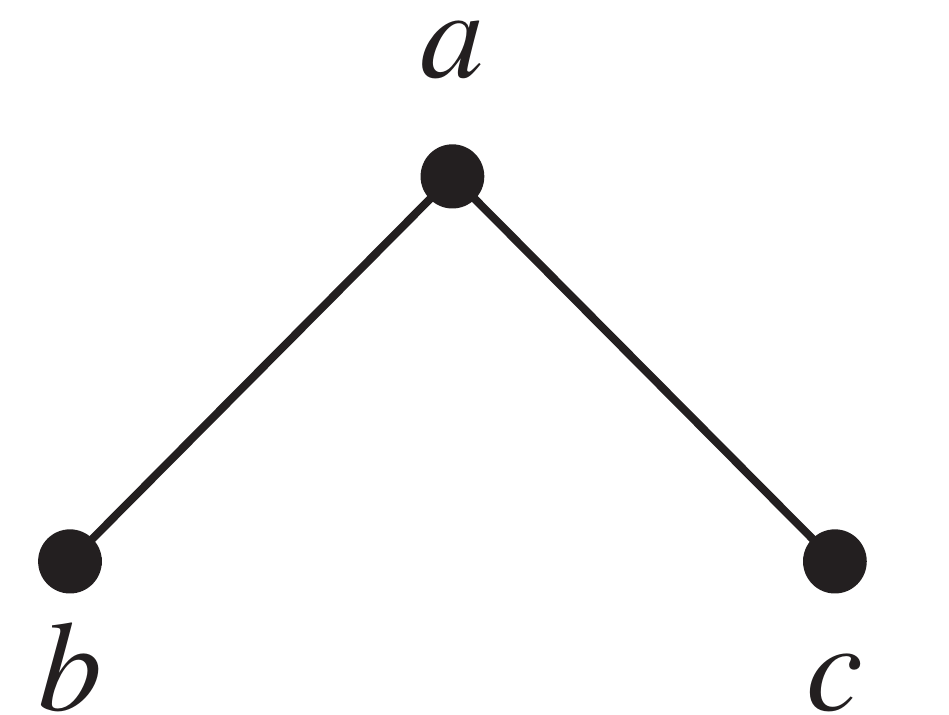
\includegraphics[scale = 0.2]{img/11_4_8_tree1.png} 
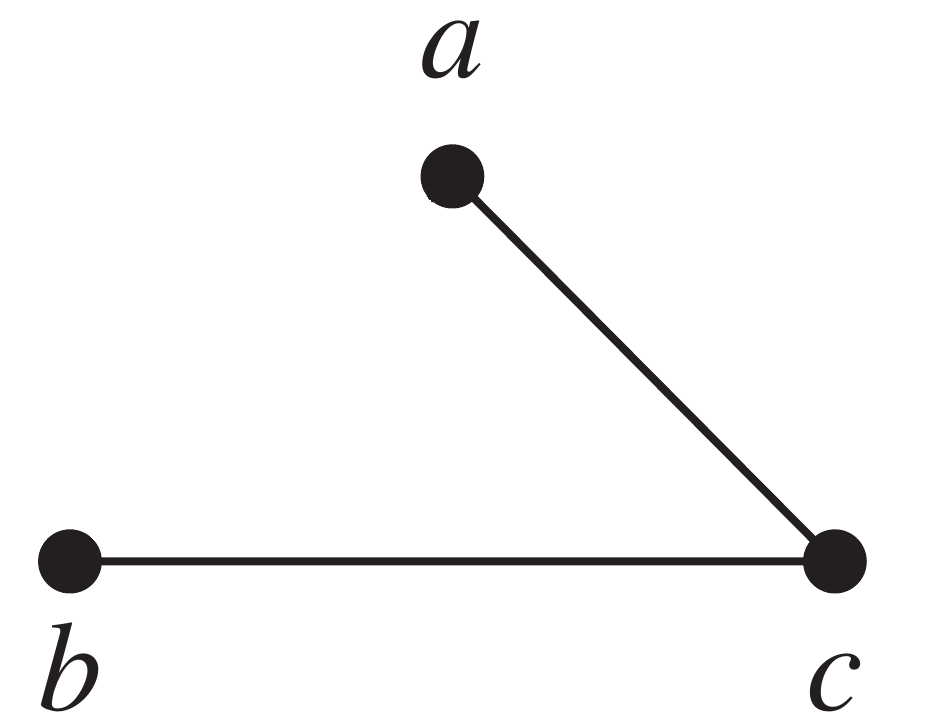
\includegraphics[scale = 0.2]{img/11_4_8_tree2.png} 
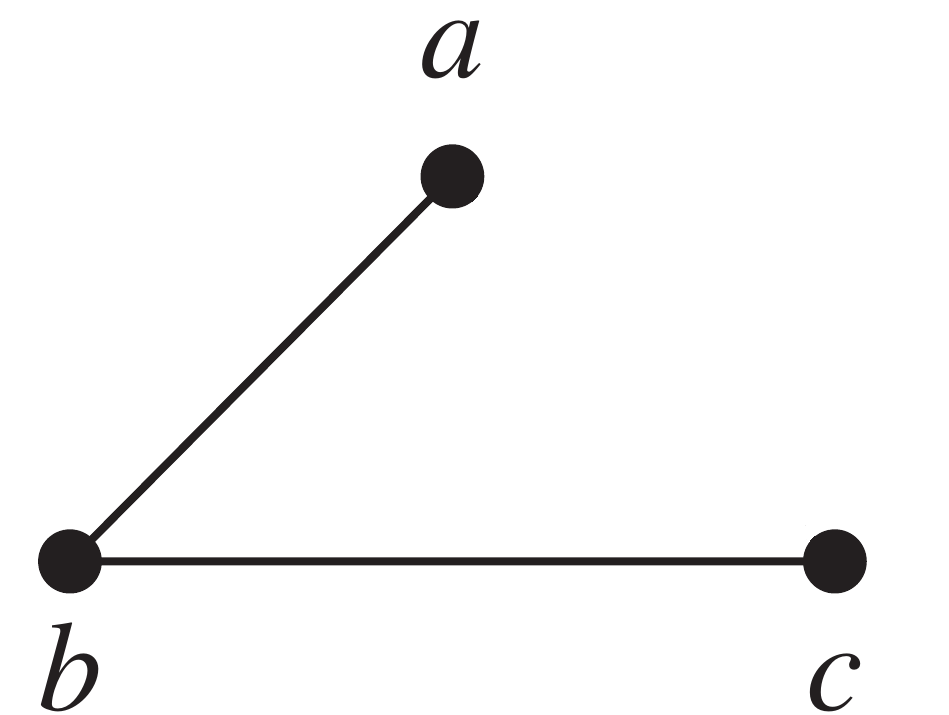
\includegraphics[scale = 0.2]{img/11_4_8_tree3.png}

\item[10.] \text{}\\
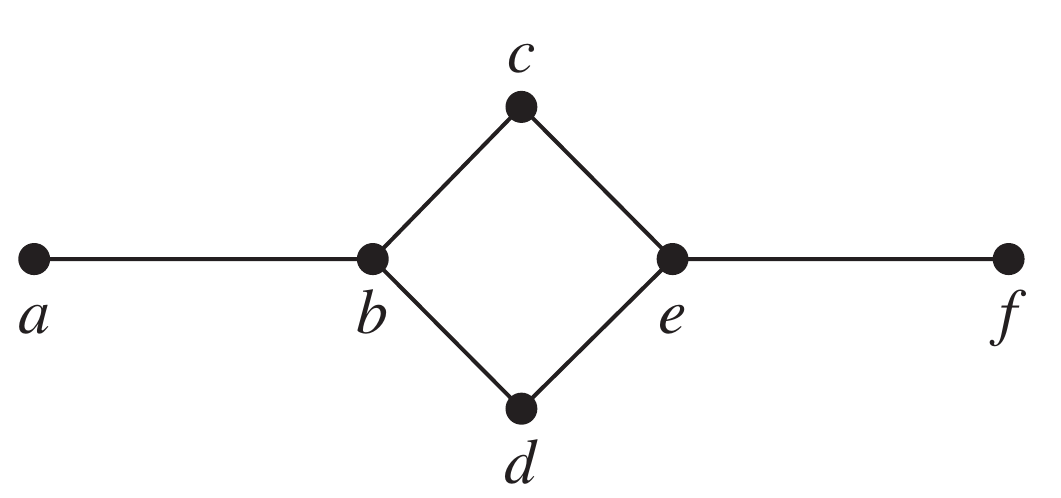
\includegraphics[scale = 0.3]{img/11_4_10_graph.png} \vspace{2mm} \\
\answer \\
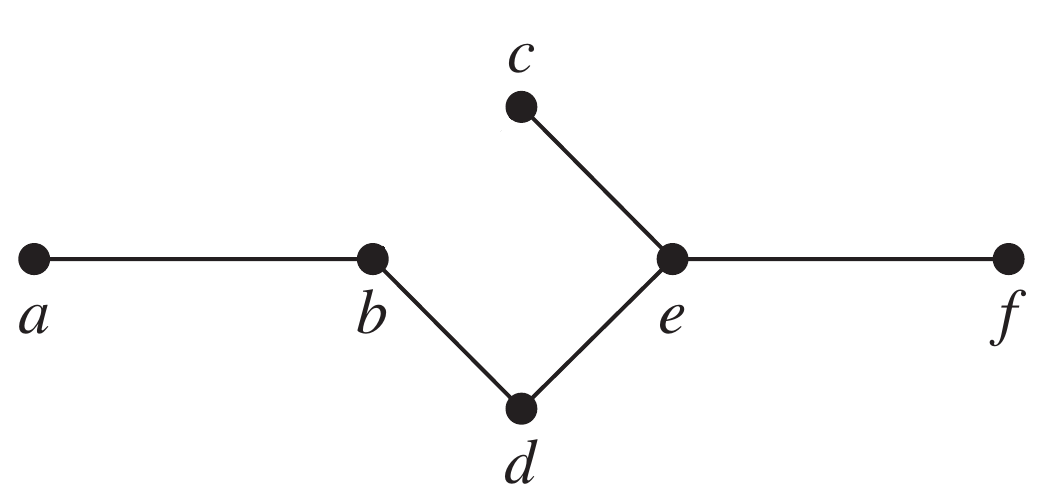
\includegraphics[scale = 0.3]{img/11_4_10_tree1.png} 
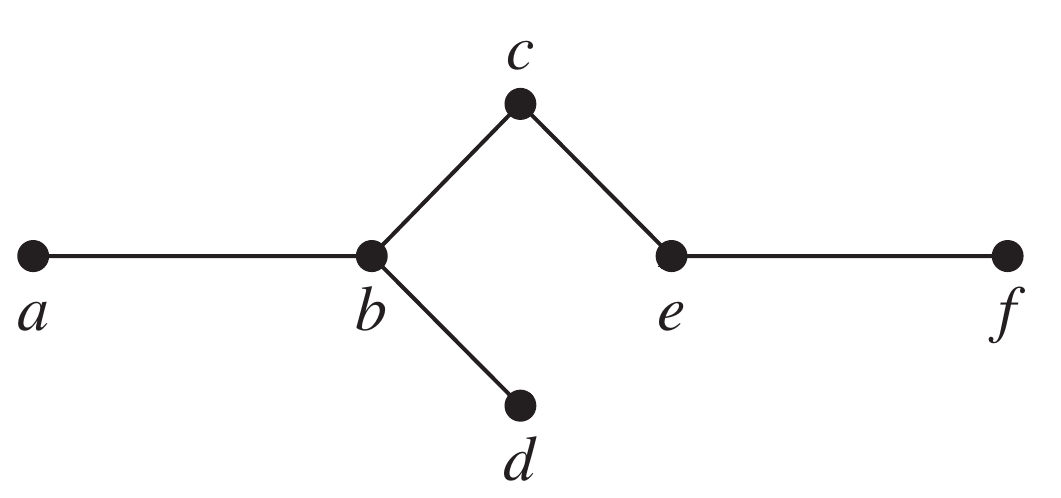
\includegraphics[scale = 0.3]{img/11_4_10_tree2.png} \\
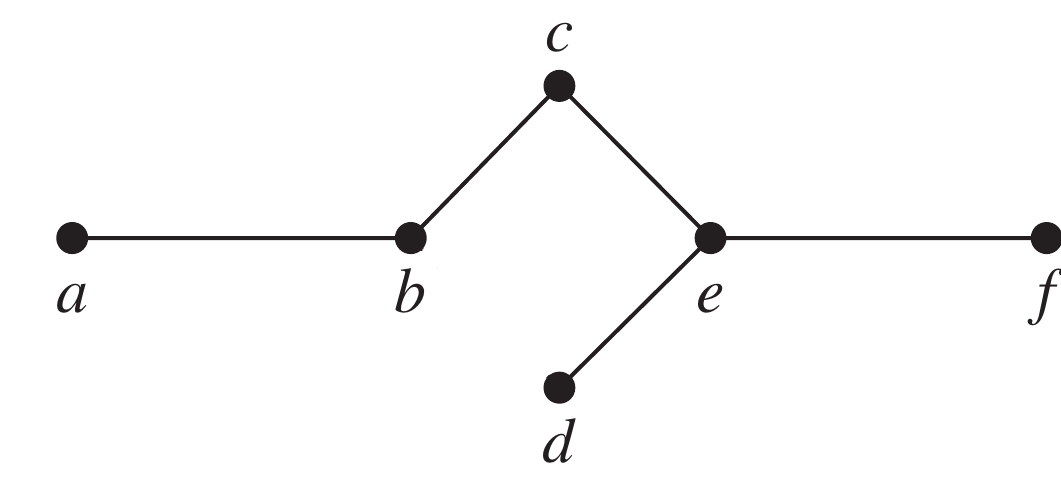
\includegraphics[scale = 0.3]{img/11_4_10_tree3.png} 
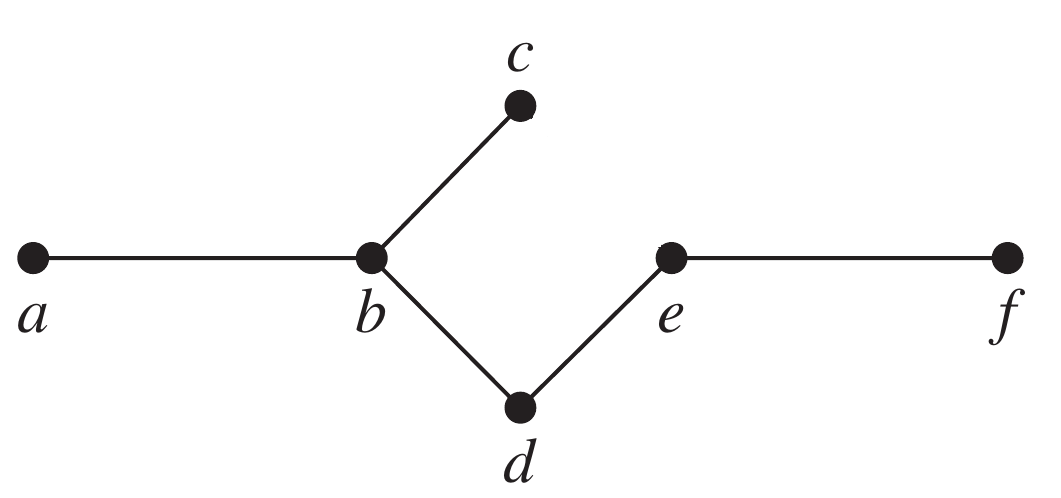
\includegraphics[scale = 0.3]{img/11_4_10_tree4.png}

\item[14.] Use depth-first search to produce a spanning tree for the given simple graph. Choose a as the root of
this spanning tree and assume that the vertices are ordered
alphabetically. \\
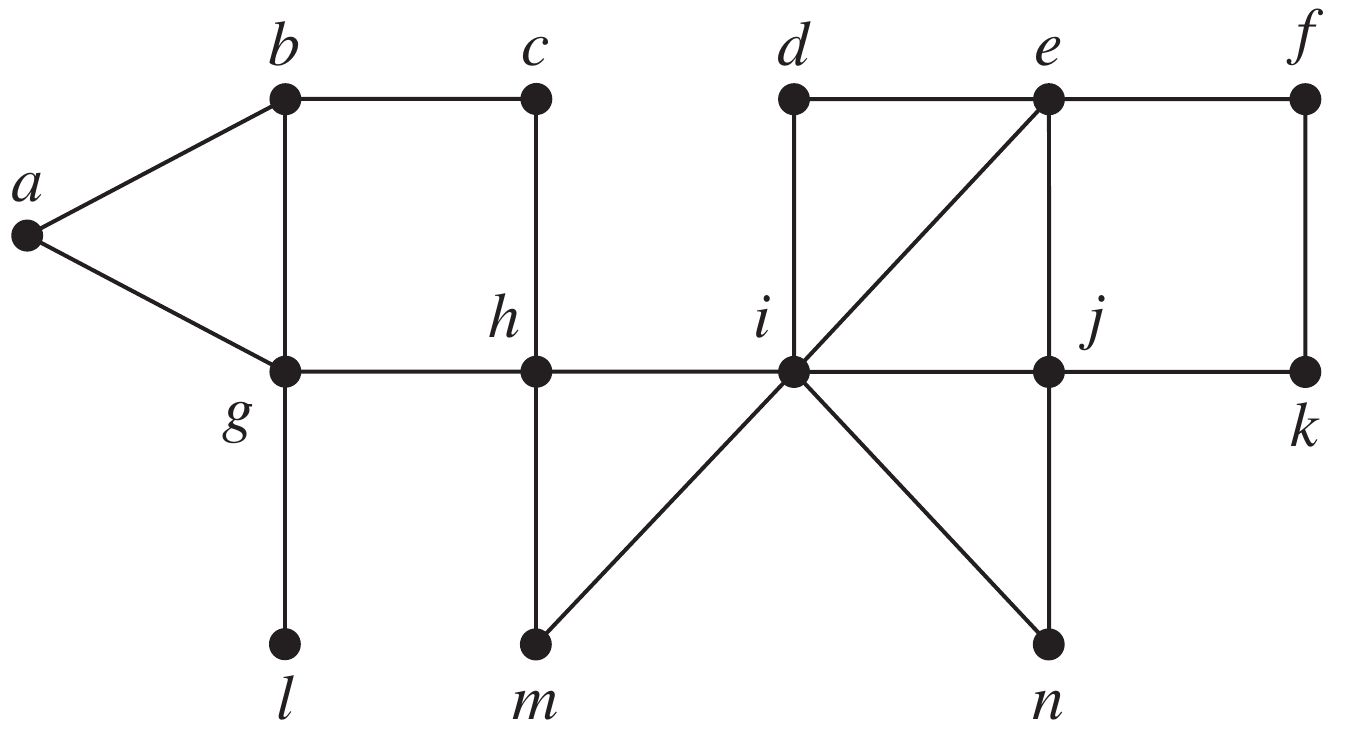
\includegraphics[scale = 0.25]{img/11_4_14_graph.png} \\
\answer \\
First start at a, then connect to b since b is before g, then connect to c, h, then g since it 
is before i and m then finally connect to l. Now return back to h and then connect 
to i then to d, e, f, k, j, n. Finally return back to i and connect to m. \\
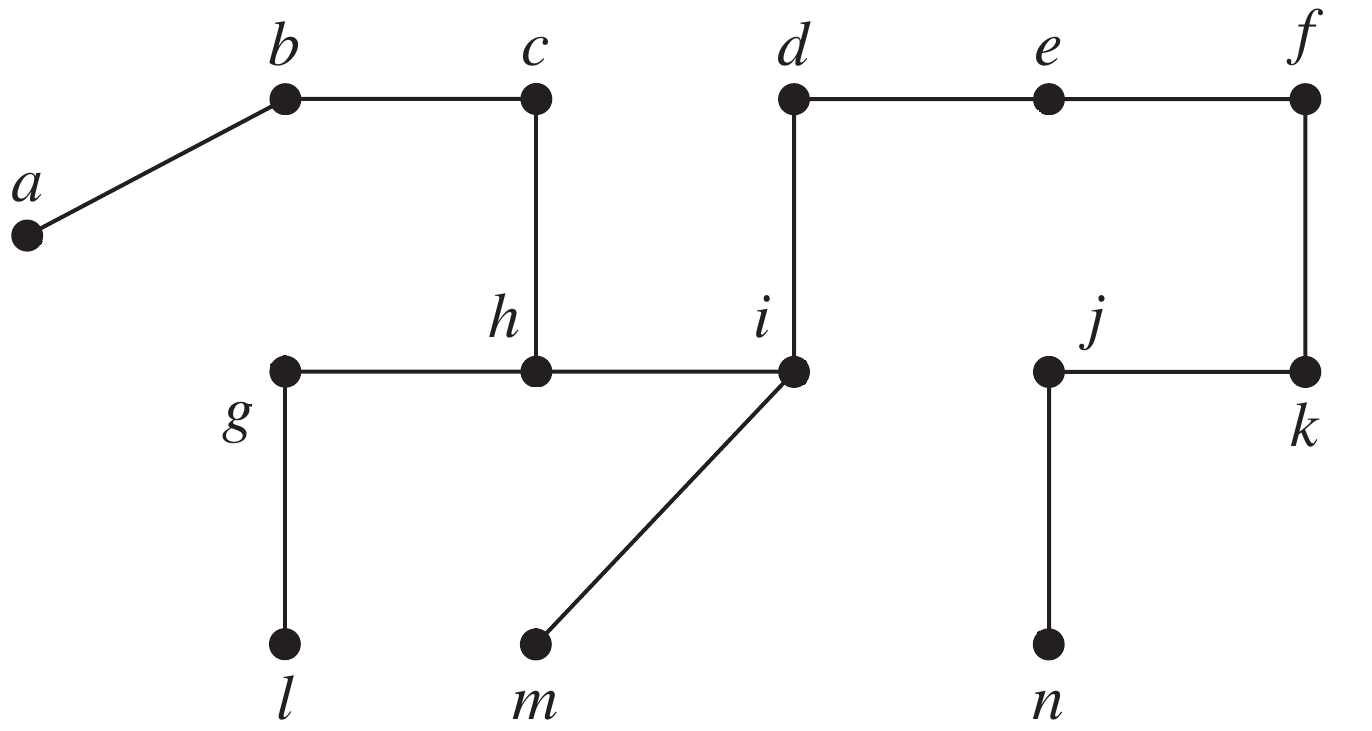
\includegraphics[scale = 0.25]{img/11_4_14_tree.png}

\item[16.]  Use breadth-first search to produce a spanning tree for
each of the simple graphs in Exercises 13–15. Choose a
as the root of each spanning tree. \\
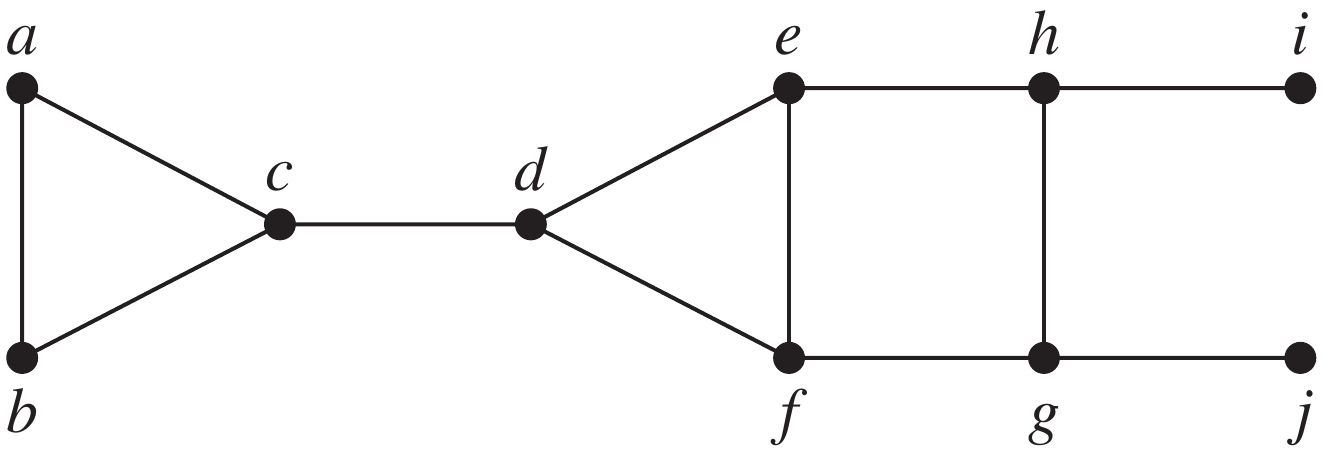
\includegraphics[scale = 0.25]{img/11_4_13_graph.png} \quad
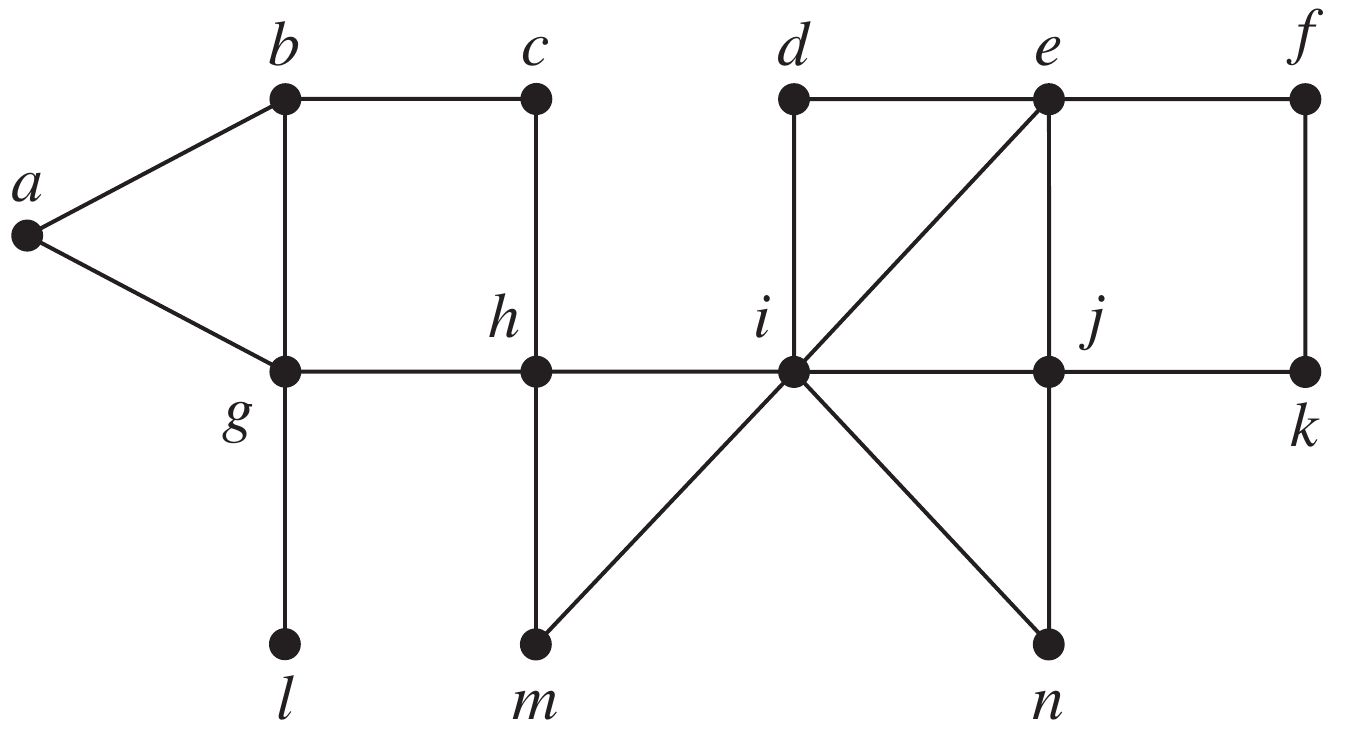
\includegraphics[scale = 0.25]{img/11_4_14_graph.png} \vspace{2mm}\\
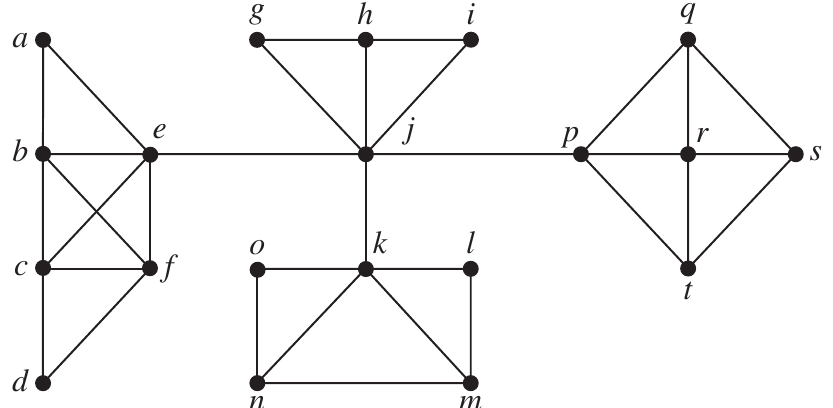
\includegraphics[scale = 0.5]{img/11_4_15_graph.png} \vspace{1.5mm}\\
\answer \\
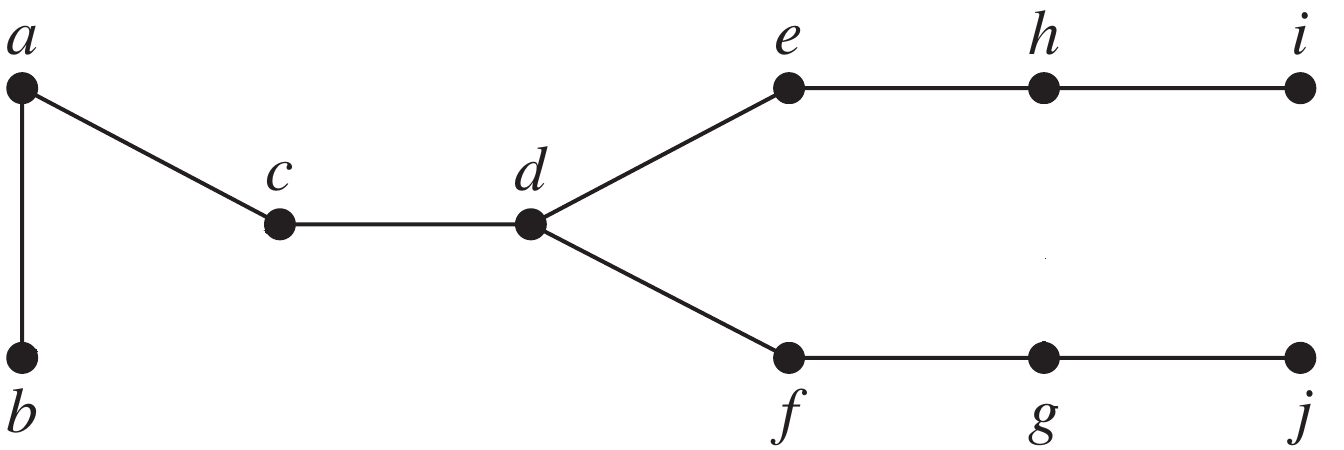
\includegraphics[scale = 0.25]{img/11_4_13_tree.png} \quad
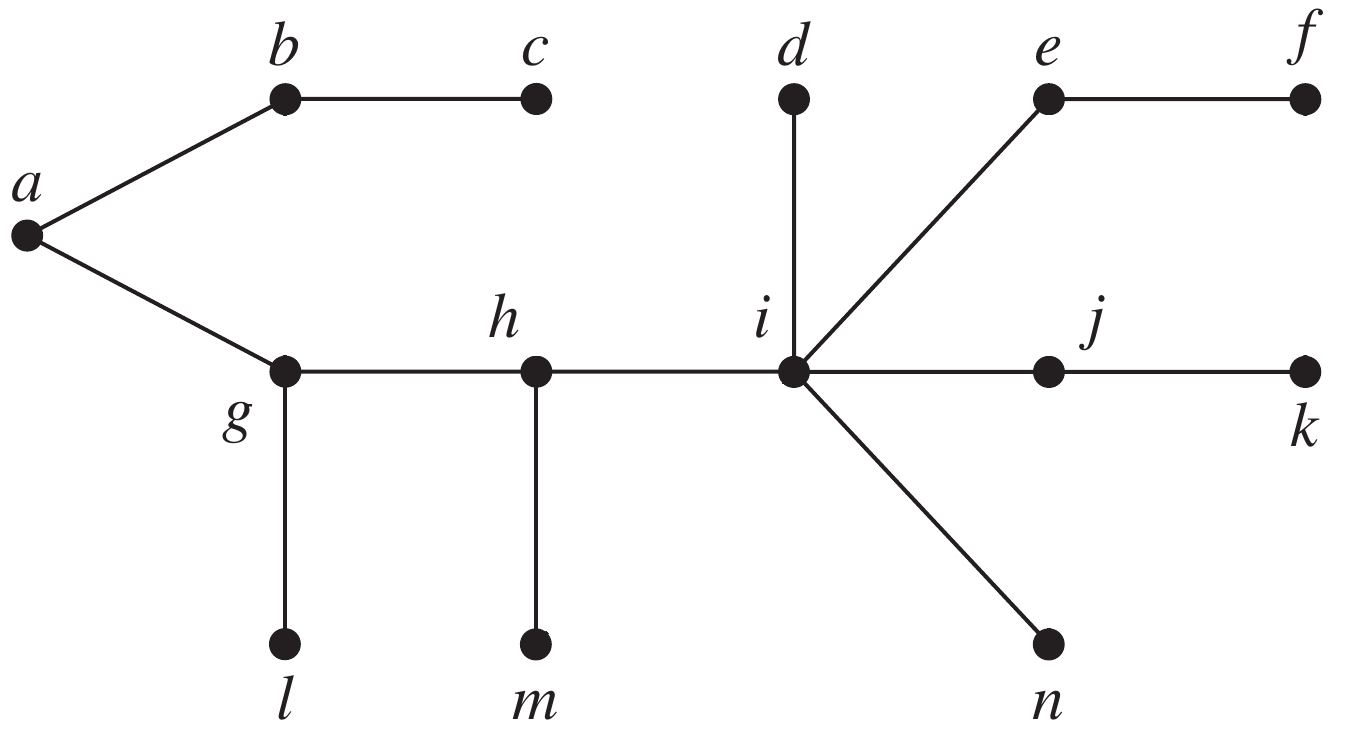
\includegraphics[scale = 0.25]{img/11_4_14_tree_bfs.png} \vspace{2mm}\\
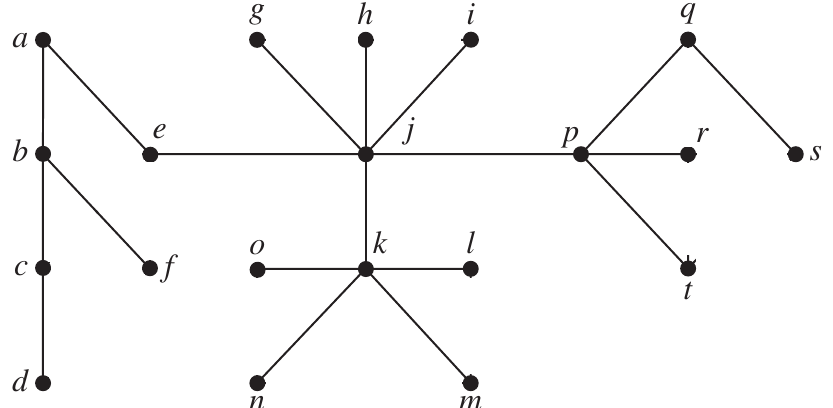
\includegraphics[scale = 0.5]{img/11_4_15_tree.png} \\

\end{itemize}

